\documentclass[tikz,border=5mm]{standalone}
\usepackage{amsmath}
\usetikzlibrary{arrows.meta, bending}

\begin{document}
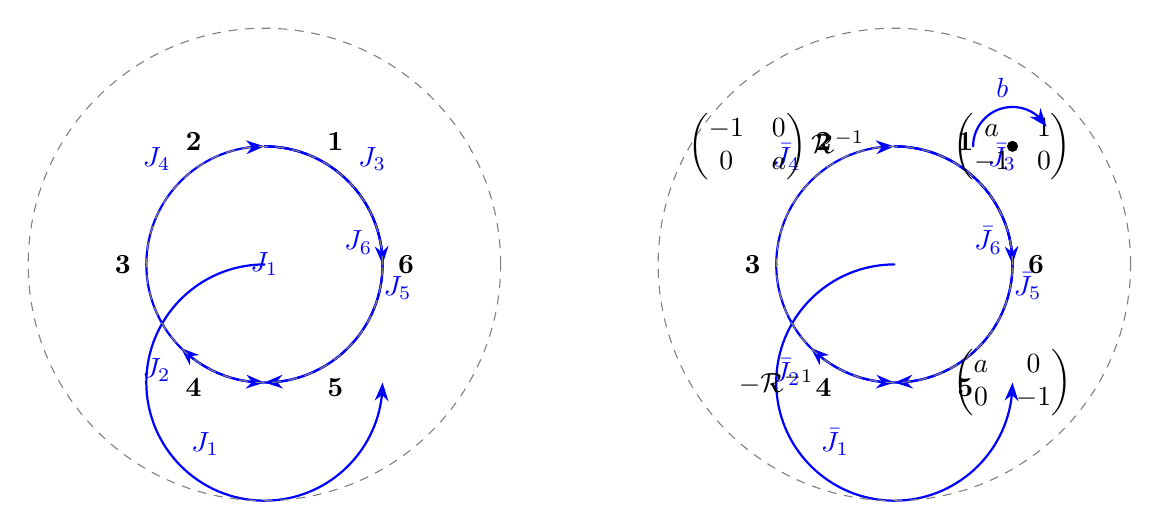
\begin{tikzpicture}[>=Stealth, line join=round, line cap=round]

% Left diagram
\begin{scope}[local bounding box=left_diagram]
    % Draw arcs
    \draw[thick, blue, ->] (0,0) arc (90:360:1.5) node[midway, above right] {$J_{1}$};
    \draw[thick, blue, ->] (0,0) ++(180:1.5) arc (180:270:1.5) node[midway, below left] {$J_{2}$};
    \draw[thick, blue, ->] (0,0) ++(90:1.5) arc (90:0:1.5) node[midway, above right] {$J_{3}$};
    \draw[thick, blue, ->] (0,0) ++(180:1.5) arc (180:90:1.5) node[midway, above left] {$J_{4}$};
    \draw[thick, blue, ->] (0,0) ++(90:1.5) arc (90:-135:1.5) node[midway, above right] {$J_{5}$};
    \draw[thick, blue, ->] (0,0) ++(90:1.5) arc (90:-90:1.5) node[midway, above left] {$J_{6}$};

    % Dotted circles
    \draw[dashed, gray] (0,0) circle (1.5);
    \draw[dashed, gray] (0,0) circle (3);

    % Number labels
    \foreach \i/\dir in {1/right, 2/left, 3/below, 4/below, 5/above, 6/above}
        \node at (\i*60:1.8) {$\mathbf{\i}$};

    % Label J_1
    \node[blue] at (0,0) {$J_{1}$};
\end{scope}

% Right diagram
\begin{scope}[shift={(8cm,0)}, local bounding box=right_diagram]
    % Draw arcs
    \draw[thick, blue, ->] (0,0) arc (90:360:1.5) node[midway, above right] {$\bar{J}_{1}$};
    \draw[thick, blue, ->] (0,0) ++(180:1.5) arc (180:270:1.5) node[midway, below left] {$\bar{J}_{2}$};
    \draw[thick, blue, ->] (0,0) ++(90:1.5) arc (90:0:1.5) node[midway, above right] {$\bar{J}_{3}$};
    \draw[thick, blue, ->] (0,0) ++(180:1.5) arc (180:90:1.5) node[midway, above left] {$\bar{J}_{4}$};
    \draw[thick, blue, ->] (0,0) ++(90:1.5) arc (90:-135:1.5) node[midway, above right] {$\bar{J}_{5}$};
    \draw[thick, blue, ->] (0,0) ++(90:1.5) arc (90:-90:1.5) node[midway, above left] {$\bar{J}_{6}$};

    % Dotted circles
    \draw[dashed, gray] (0,0) circle (1.5);
    \draw[dashed, gray] (0,0) circle (3);

    % Number labels
    \foreach \i/\dir in {1/right, 2/left, 3/below, 4/below, 5/above, 6/above}
        \node at (\i*60:1.8) {$\mathbf{\i}$};

    % Matrices
    \node at (-1.5,1.5) {$\begin{pmatrix} -1 & 0 \\ 0 & a \end{pmatrix}\mathcal{R}^{-1}$};
    \node at (1.5,-1.5) {$\begin{pmatrix} a & 0 \\ 0 & -1 \end{pmatrix}$};
    \node at (-1.5,-1.5) {$-\mathcal{R}^{-1}$};
    \node at (1.5,1.5) {$\begin{pmatrix} a & 1 \\ -1 & 0 \end{pmatrix}$};

    % Dot and arrow
    \fill[black] (1.5,1.5) circle (2pt);
    \draw[blue, ->, >=Stealth, thick] (1.5,1.5) ++(180:0.5) arc (180:30:0.5) node[midway, above] {$b$};
\end{scope}

\end{tikzpicture}
\end{document}